\documentclass[a4j,12pt,dvipdfmx]{jsreport}

% 数式
\usepackage{amsmath,amsfonts}
\usepackage{bm}

% 画像
\usepackage[dvipdfmx,top=35truemm,bottom=30truemm,left=30truemm,right=30truemm]{geometry}
\usepackage[dvipdfmx]{graphicx}
% biblatex
\usepackage[style=numeric, sorting=none, maxbibnames=1000]{biblatex}
\addbibresource{graduation_thesis.bib}

% itembox
\usepackage{ascmac}
% breakitemboxのためのpackage
\usepackage{itembkbx}
% \usepackage{tcolorbox} 画像が見えなくなってしまう原因
% \usepackage{framed} 枠

% フォント
\usepackage[ipaex]{pxchfon}
\listfiles
\usepackage{float}
\usepackage{multicol}
\usepackage{multirow}
\usepackage{paralist}
\usepackage{caption}
% \captionsetup{format=plain, justification=centering}
\usepackage{setspace}
\usepackage{algorithm}
\usepackage{algpseudocode}
\usepackage[dvipdfmx,hidelinks]{hyperref}
\usepackage{pxjahyper}
\usepackage{fancyhdr}
\usepackage{ltablex}
\usepackage{capt-of}
\usepackage{tabularx}
\usepackage{adjustbox}
\usepackage{booktabs}
\usepackage{enumitem} % itemizeの行間 これは下になければならない
\usepackage{threeparttable} % 表の脚注
\usepackage{titlesec}
\usepackage{makecell}
% titlesec と \paragraph の相性問題を回避（run-in 見出しにする）
\titleformat{\paragraph}[runin]
  {\normalfont\normalsize\bfseries}
  {}{0pt}{} % ←ここには文字や \noindent 等を入れない
\titlespacing*{\paragraph}
  {0pt}{1.0ex}{0.8em}
\titleformat{\chapter}[hang]{\LARGE\bfseries}{\prechaptername\thechapter\postchaptername}{1em}{}

\setlength{\headheight}{16.5pt}
\captionsetup{format=hang}
\captionsetup[figure]{font=small}
\captionsetup[table]{font=small}
\begin{document}

% ▼▼▼ 仕掛け：main じゃないとき（単体のとき）だけヘッダー設定 ▼▼▼
\ifdefined\ismain\else
  \pagestyle{fancy}
  \lhead{\rightmark}
  \renewcommand{\chaptermark}[1]{\markboth{第\ \thechapter\ 章\ #1}{}}
  \setlength{\headheight}{16.5pt}
  \titleformat{\chapter}[hang]{\LARGE\bfseries}{\prechaptername\thechapter\postchaptername}{1em}{}
\fi
% ▲▲▲▲▲▲▲▲▲▲▲▲▲▲▲▲▲▲▲▲▲▲▲▲▲▲▲▲▲▲▲▲▲▲▲▲

\chapter{脚本に基づく漫画のレイアウト生成}\label{chap:script2layout}

本章では，前章で構築した Manga109ScriptDataset を用い，
脚本に基づいて漫画ページ内のレイアウトを生成する手法（Script2Layout）について述べる．
ここで扱うレイアウト生成とは，
コマ，キャラクター，およびセリフを要素とし，
それらの平面上での配置をページ単位で予測するタスクである．

本研究における漫画のネーム生成は，
脚本に基づいてレイアウトおよび演出情報を生成する問題として位置づけている．
そのうち本章は，
物語内容を含む脚本情報が，
要素配置という幾何学的なレイアウト決定に対して
どの程度有効に機能するかを検証することを目的とする．
これは，後続章で扱う演出情報を含むネーム生成に先立ち，
脚本情報を条件とした生成モデルの基礎的な挙動を明らかにする段階に相当する．

本章の構成は以下の通りである．
まず~\ref{sec:problem_formulation}節では，
脚本に基づく漫画レイアウト生成タスクの問題設定を定式化する．
次に~\ref{sec:method}節において，
脚本情報を入力に利用するレイアウト生成手法(Script2Layout)の概要を述べる．
~\ref{sec:experimental_setup}節では，
使用したデータセット，評価指標，および比較手法を含む実験設定について説明する．
続いて~\ref{sec:results}節で定量的な評価および定性的な評価の結果を示し，これらについて考察する．


\section{漫画のレイアウト生成における問題設定}\label{sec:problem_formulation}

本章では，脚本に基づく漫画レイアウト生成を，
漫画ページ内に配置される各要素の
二次元平面上での位置と大きさを予測する問題として定式化する．
ここで扱うレイアウト要素は，
キャラクター，セリフのフキダシ，およびコマであり，
これらはいずれも漫画のネームの中で
物語内容に応じて配置が設計される主要な構成要素である．

漫画ページ上のレイアウトは，
$N \in \mathbb{N}$ 個の要素からなる集合として表され，
これを
\begin{equation}
  \ell = \{(c_1, \mathbf{b}_1), \dots, (c_N, \mathbf{b}_N)\}
\end{equation}
と定義する．
ここで $c_i$ は $i$ 番目の要素を識別するカテゴリを表し，
本研究においては，
キャラクター，セリフのフキダシ，コマ
を基本要素種別とし，さらにキャラクターとセリフにおいてはそれらがどのキャラクターに属するかという区別まで含んだ識別子として定義される．
つまり，$c_i$ は，
要素の基本種別とキャラクター種別に基づいて定義される
カテゴリ集合 $\mathcal{C}$ の要素であり，$\mathcal{C}$ は
\begin{equation}
  \mathcal{C}
  =
  \{\text{panel}\}
  \;\cup\;
  \{\text{character}_k\}
  \;\cup\;
  \{\text{speech}_k\}
\end{equation}
と表されるものとする．
ここで $\text{character}_k$ はページ内に登場する
第 $k$ 番目のキャラクターに対応するキャラクター要素を表し，
$\text{speech}_k$ は同キャラクターによる発話に対応する
セリフのフキダシ要素を表す．$\mathbf{b}_i$ はその要素に対応するバウンディングボックスであり，
ページ平面上における位置と大きさを表す
矩形領域として定義される．


以上の定義のもと，
本研究におけるレイアウト生成タスクは，
要素数 $N$ と対応するカテゴリ集合
$\{c_i\}_{i=1}^{N}$ が与えられたとき，
それぞれの要素に対応する
バウンディングボックス
$\{\mathbf{b}_i\}_{i=1}^{N}$ を予測する問題として定式化される．
この設定は，
漫画制作において，物語の決定とともに
各ページに登場するキャラクターやセリフが定まり，
それらをどのように配置するか設計する
ネーム作成の工程に対応している．

既存のレイアウト生成手法では，
このようなカテゴリが
事前に記号的なラベルとして与えられることを前提としていた．
これに対し本研究では，
キャラクター名やセリフ内容といった
脚本に含まれる言語情報を入力に利用し，
それらを条件としてレイアウトを生成する設定を採用する．
このように，
物語内容を含む脚本情報を条件としたレイアウト生成を扱うことで，
物語的意図が
ページ上の配置決定にどのように反映され得るかを検証する．

以下では，
この問題設定に基づき，
脚本情報を直接入力として利用する
レイアウト生成手法(Script2Layout)について述べる．


\section{脚本に基づく漫画のレイアウト生成手法}\label{sec:method}
本節では，脚本情報を条件として漫画ページのレイアウトを生成する手法
Script2Layout の概要を述べる．
図\ref{fig:script2layout_overview} に，
本研究で扱う手法の全体像を示す．

\begin{figure}[htbp]
  \centering
  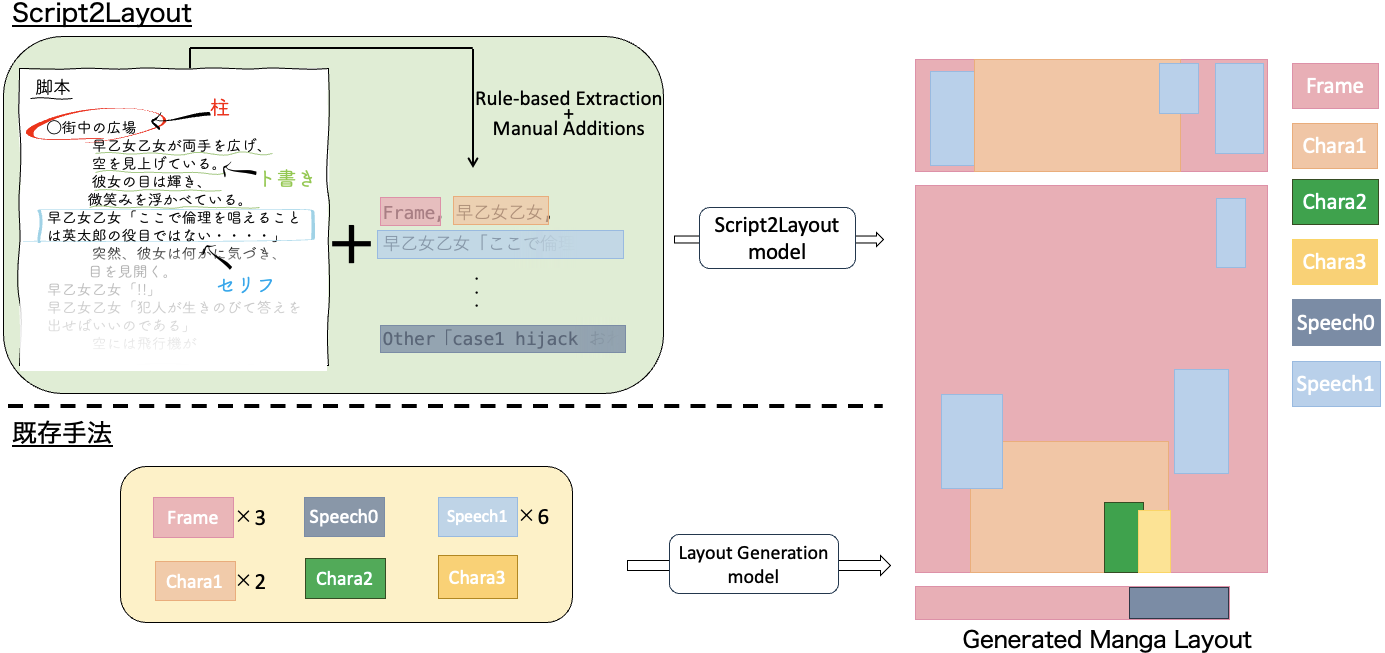
\includegraphics[width=\textwidth]{pict/04/script2layout_inputoutput.png}

  \caption{
    Script2Layout による脚本条件付きレイアウト生成の概略図．
    上段は，本研究で提案する手法であり，
    自然言語として記述された脚本を直接入力として扱いつつ，
    キャラクター，セリフ，およびコマに対応する要素を抽出し，
    Fine-tuned LLM によりページ全体のレイアウトを生成する．
    下段は，既存のレイアウト生成手法の例であり，
    要素数やカテゴリといった構造化情報を入力として
    レイアウトを生成する点で異なる．
  }
  \label{fig:script2layout_overview}
\end{figure}

本研究におけるScript2Layoutは，
脚本に基づく漫画レイアウト生成タスクに対し，LLMを
教師あり学習によりファインチューニングする形で構築した．

前節で定義した通り，
漫画ページのレイアウトは，
カテゴリとバウンディングボックスの組からなる集合
\begin{equation}
  \ell = \{(c_1, \mathbf{b}_1), \dots, (c_N, \mathbf{b}_N)\}
\end{equation}
として表される．
本研究では，
ページ単位の脚本を自然言語列 $S$ とし，脚本に基づく漫画のレイアウト生成タスクを，
$S$に対応するレイアウト $\ell$ を生成する
条件付き生成問題として定式化する．
すなわち，
脚本 $S$ が与えられたもとで，
レイアウトを構成する各要素の
カテゴリに対応した配置情報を出力する写像を学習する．

LLM による生成および学習を可能にするため，
レイアウト集合 $\ell$ に含まれる
各要素 $(c_i, \mathbf{b}_i)$ を，
あらかじめ定めた順序に従って線形化し，
トークン列として表現する．
具体的には，
\begin{equation}
  L = (l_1, l_2, \dots, l_T)
\end{equation}
をレイアウト列とし，
各トークン $l_t$ は
単一のレイアウト要素に対応するものとして
\begin{equation}
  l_t = (c_{\pi(t)}, \mathbf{b}_{\pi(t)})
\end{equation}
と定義する．
ここで $\pi(t)$ は，
集合 $\ell$ に含まれる要素を
系列上の位置 $t$ に対応付ける写像であり，
ページ内の全要素を一度ずつ列挙するため，
$T = N$ が成り立つ．

各要素に対応するバウンディングボックス
$\mathbf{b}_i = (x_i, y_i, w_i, h_i)$ は，
ページ平面上での位置と大きさを表す連続値である．
本研究では，
これらをあらかじめ定義した二次元の格子点上に量子化し，
有限語彙上の離散トークンとして表現する．
これにより，
レイアウト生成は
有限語彙上の系列生成問題として定式化され，
LLM の自己回帰的な生成枠組みと
直接的に対応付けて扱うことが可能となる．

入力となる脚本 $S$ には，
柱，ト書き，およびセリフを含む
ページ単位の脚本全文を自然言語としてそのまま与える．
本研究では，
キャラクター名を正規化することを行わず，
脚本中に現れる表記をそのまま入力として用いる．
一方で，
セリフは「話者名『発話内容』」の形式で記述されているため，
モデルは話者と発話内容の対応関係や，
ト書きに記述された振る舞いを
条件情報として利用できる．
これにより，
どのキャラクターがページ内で中心的であるか，
どのキャラクターに発話が集中しているかといった
物語構造が，
レイアウト生成の手がかりとしてモデルに与えられる．

学習時には，
脚本列 $S$ と，
それに対応する正解レイアウト列 $L$ からなる
教師データを用い，
LLM による条件付き確率
\begin{equation}
  p_{\theta}(L \mid S)
  =
  \prod_{t=1}^{T}
  p_{\theta}(l_t \mid l_{<t}, S)
\end{equation}
を最大化するように，
モデルパラメータ $\theta$ を最適化する．
具体的には，
次トークン予測に基づく
クロスエントロピー損失
\begin{equation}
  \mathcal{L}
  =
  - \sum_{t=1}^{T}
  \log p_{\theta}(l_t \mid l_{<t}, S)
\end{equation}
を最小化することで，
脚本とレイアウトとの対応関係を
モデル内部に学習させる．

このような教師ありファインチューニングを通じて，
LLM は，
自然言語として記述された物語情報と，
漫画ページ上の幾何的な配置との対応関係を，
明示的なルール設計に依存することなく獲得する．
既存のレイアウト生成手法の多くが，
要素カテゴリやサイズといった
構造化された入力を前提としていたのに対し，
本研究では，
脚本そのものを入力として利用し，
LLM の言語理解能力を介して
配置決定を行う点に特徴がある．

以上のように，
LLM を脚本条件付きのレイアウト生成器として
教師ありでファインチューニングすることで，
物語内容に基づく配置設計を
一貫した生成モデル，Script2Layoutとして実現する．

\section{漫画のレイアウト生成における実験設定}\label{sec:experimental_setup}

本節では，
前節で述べた Script2Layout 手法の有効性を検証するために行った
実験設定を述べる．
具体的には，
データセット分割，
比較手法，
制約条件，
評価指標，
実装詳細を順に説明する．

\subsection{データセット分割}

実験には本研究において構築した Manga109ScriptDataset を用いる．
制約条件，特に要素間関係を用いる設定において
計算量が大きくなるケースを避けるため，
ページ内の総要素数が 50 を超えるページを除外し，
残る 19,465 ページを実験対象とした．

データは作品単位で分割し，
同一作品が訓練用・検証用・テスト用データにまたがらないようにした．
分割比は 8:1:1 とし，
訓練用データを 15,386 ページ，検証用データを 2,183 ページ，テスト用データを 1,896 ページ用いた．
訓練用データは Script2Layout のファインチューニングおよび
比較手法の学習に用い，
検証用データは学習の早期終了等のモデル選択に用いた．
最終的な性能評価はテスト用データ上で行った．
\subsection{比較手法}

Script2Layout は脚本を条件としてレイアウトを生成するのに対し，
既存のレイアウト生成手法は，
要素カテゴリが記号的ラベルとして与えられることを前提とする．
そこで比較実験では，
既存手法に合わせて各ページ内の要素カテゴリをラベル化し，
同一の入出力形式で性能比較を行った．

既存手法の入力カテゴリは，
ページ内のコマを $\texttt{Panel}$，
キャラクターを $\texttt{Character}_k\ (k=1,\dots,25)$，
セリフのフキダシを $\texttt{Speech}_k\ (k=0,\dots,25)$
として定義する．
ここで $k$ はページ内で区別されるキャラクター種別を表し，
$\texttt{Speech}_k$ は $\texttt{Character}_k$ による発話に対応する．
また $k=0$ は独立したナレーション等話者が特定できないものを表す．
キャラクター種別数の最大値を25としたのは，本データセットで単一ページ内に登場するキャラクター種別数の最大値が22であることから余裕をもたせたものである．

比較対象として，
LayoutDM~\cite{inoue_layoutdm_2023}，
LayoutFormer++~\cite{jiang_layoutformer_2023}，
LayoutPrompter~\cite{lin_layoutprompter_2023}
の 3 手法を採用した．
LayoutDM と LayoutFormer++ は学習型モデルであり，
本データセットの訓練分割を用いて 0 から学習させた．
LayoutPrompter は GPT-4o を利用するプロンプトベースの手法であり，
学習は行わず推論のみを用いた．
なお LayoutPrompter は入力長の制約のため
脚本全文を条件として与えない設定で評価した．

\subsection{制約条件}
既存の手法が扱う制約条件からは以下のものを採用した．

\begin{itemize}
  \item \textbf{Gen-T（types 条件）:}
        各要素のカテゴリ（$\texttt{Panel}$，$\texttt{Chara}_k$，$\texttt{Speech}_k$）のみを与え，
        バウンディングボックスを生成する条件．本章の基本設定とする．
  \item \textbf{Gen-TS（types+sizes 条件）:}
        各要素のカテゴリに加え，
        バウンディングボックスのサイズ（幅・高さ）を与え，
        位置のみを生成する条件．
\end{itemize}

一方 Script2Layout では，
前節の通り脚本を自然言語として入力に含めることができる．
脚本条件の効果を検証するため，
Script2Layout は入力形式を以下の 2 通り比較した．

\begin{itemize}
  \item \textbf{Without Script:}   脚本全文は入力に含めず，
        キャラクター名やセリフ内容といった
        各要素のテキスト情報のみを入力として用いる条件．
        この条件においても，
        Script2Layout モデルは同一の学習データを用いて
        教師ありでファインチューニングされている
  \item \textbf{With Script:} ページ単位で脚本全文を自然言語としてそのまま与える条件．
\end{itemize}

それぞれの条件を，比較手法の Gen-T，Gen-TS と組み合わせて実験を行った．

\subsection{評価指標}\label{sec:metrics}
漫画レイアウトは同一脚本に対しても複数の妥当な解が存在し得るため，
単一の観点だけで生成品質を評価することは難しい．
そこで本研究では，
(1) 生成結果の分布としての近さ，
(2) 要素単位での位置精度，
(3) ページ単位での集合としての幾何的一致，
(4) データ集合としての幾何的一致
をそれぞれ測るため，
Fréchet Inception Distance(FID)，Mean Intersection over Union (mIoU)，Layout Transportation Similarity（LTSim）~\cite{otani_ltsim_2024}，LTSim Maximum Mean Discrepancy（LTSim-MMD）~\cite{otani_ltsim_2024} の4指標を用いる．
特に LTSim は最適輸送に基づく柔軟な要素対応付けにより，
要素数やカテゴリの差異を含むレイアウト対も比較可能な指標として提案されている~\cite{otani_ltsim_2024}．
また，FID は分布比較に広く用いられる一方で，
知覚品質と必ずしも一致しない可能性も指摘されているため~\cite{otani_ltsim_2024}，
本研究では LTSim 系指標を併用して多面的に評価する．

\par
\paragraph{FID}
生成レイアウトと実レイアウトの分布の近さを測るため，
Fréchet Inception Distance（FID）を用いる．
FID は，レイアウトを特徴空間へ写像した後，生成分布と実分布を
それぞれ多変量正規分布として近似し，
その間の Fréchet 距離として定義される：
\begin{equation}
  \mathrm{FID}
  =
  \|\boldsymbol{\mu}_g - \boldsymbol{\mu}_r\|_2^2
  +
  \mathrm{Tr}
  \left(
  \boldsymbol{\Sigma}_g
  +
  \boldsymbol{\Sigma}_r
  -
  2(\boldsymbol{\Sigma}_g \boldsymbol{\Sigma}_r)^{1/2}
  \right),
\end{equation}
ここで $(\boldsymbol{\mu}_g, \boldsymbol{\Sigma}_g)$ および
$(\boldsymbol{\mu}_r, \boldsymbol{\Sigma}_r)$ は，
それぞれ生成レイアウトと実レイアウトから抽出した特徴の
平均および共分散行列である．
特徴抽出器には LayoutDM~\cite{inoue_layoutdm_2023} に倣い
FIDNetV3 を用いる．

\paragraph{mIoU}
生成された各レイアウト要素と正解要素を
カテゴリごとに一対一で対応付け，
それらの Intersection over Union（IoU）を評価する．
要素 $i$ に対する IoU は，
生成バウンディングボックス $\mathbf{b}_i^{(g)}$ と
正解バウンディングボックス $\mathbf{b}_i^{(r)}$ に対して
\begin{equation}
  \mathrm{IoU}_i
  =
  \frac{
    \mathrm{area}
    \left(
    \mathbf{b}_i^{(g)} \cap \mathbf{b}_i^{(r)}
    \right)
  }{
    \mathrm{area}
    \left(
    \mathbf{b}_i^{(g)} \cup \mathbf{b}_i^{(r)}
    \right)
  }
\end{equation}
として定義される．
同一カテゴリ内で IoU が最大となる対応を貪欲に選択し，
全要素に対する平均値
\begin{equation}
  \mathrm{mIoU}
  =
  \frac{1}{N}
  \sum_{i=1}^{N} \mathrm{IoU}_i
\end{equation}
を最終的な指標として算出する．

\paragraph{LTSim}
ページ単位での幾何的一致を評価するため，
最適輸送に基づく Layout Transportation Similarity（LTSim）~\cite{otani_ltsim_2024} を用いる．
LTSim は，
生成レイアウト $\hat{\ell}$ と正解レイアウト $\ell$ に含まれる要素集合を，
一対一に対応付けるのではなく，
要素間の類似度に基づく重み付きの多対多対応（ソフト対応）として扱う点に特徴がある．

具体的には，
正解レイアウト $\ell=\{(c_i,\mathbf{b}_i)\}_{i=1}^{N}$ と
生成レイアウト $\hat{\ell}=\{(c_j,\hat{\mathbf{b}}_j)\}_{j=1}^{\hat{N}}$
の間に，
輸送行列 $\gamma \in \mathbb{R}_{+}^{N \times \hat{N}}$ を導入し，
各要素対 $(i,j)$ の対応の強さを $\gamma_{i,j}$ として表す．
$\gamma$ は各要素の総重みを保存する制約のもとで最適化され，
要素数やカテゴリが完全に一致しない場合でも対応付けが可能である．

このとき，
対応に基づく輸送コスト（Earth Mover's Distance; EMD）は
\begin{equation}
  \mathrm{EMD}(\ell,\hat{\ell})
  =
  \sum_{i=1}^{N}\sum_{j=1}^{\hat{N}}
  \gamma^\ast_{i,j}\,
  \mu\bigl((c_i,\mathbf{b}_i),(c_j,\hat{\mathbf{b}}_j)\bigr)
\end{equation}
として定義される．
ここで $\gamma^\ast$ は輸送コストを最小化する最適輸送行列であり，
$\mu(\cdot,\cdot)$ は要素間のコスト関数である．
本研究では，
$\mu$ として
バウンディングボックス間の幾何的差異を表す Generalized IoU（GIoU）と，
カテゴリ一致の有無を組み合わせたコストを用いる~\cite{otani_ltsim_2024}．
これにより，
位置関係と要素種別の両方を考慮した対応付けが実現される．

EMD に基づき，
LTSim は次式で定義される：
\begin{equation}
  \mathrm{LTSim}(\ell,\hat{\ell})
  =
  \exp\!\left(-\frac{\mathrm{EMD}(\ell,\hat{\ell})}{\sigma}\right).
\end{equation}
$\sigma$ はスケールパラメータであり，
EMD の大きさを類似度に変換する際の感度を制御する．
本研究では，
1ページ全体を1つのレイアウトとして比較する
layout-level の設定に従い，
$\sigma=1$ とする~\cite{otani_ltsim_2024}．


\paragraph{LTSim-MMD}
生成レイアウト集合と実レイアウト集合の分布的一致を評価するため，
LTSim をカーネル関数とする
Maximum Mean Discrepancy（MMD）に基づく
LTSim-MMD~\cite{otani_ltsim_2024} を用いる．

MMD は，
2つの集合が同一の分布から生成されたかどうかを評価する指標であり，
集合内および集合間の平均類似度の差に基づいて定義される．
本研究では，
ページ単位のレイアウト間類似度として LTSim を用い，
これをカーネル関数
$k(\ell,\hat{\ell})=\mathrm{LTSim}(\ell,\hat{\ell};\sigma)$
として用いる．

正解レイアウト集合 $\mathcal{L}=\{\ell_i\}_{i=1}^{s}$ と
生成レイアウト集合 $\hat{\mathcal{L}}=\{\hat{\ell}_j\}_{j=1}^{t}$ に対し，
LTSim-MMD は
\begin{equation}
  \mathrm{MMD}^2(\mathcal{L},\hat{\mathcal{L}})
  =
  \frac{1}{s(s-1)}\sum_{i\neq j} k(\ell_i,\ell_j)
  +
  \frac{1}{t(t-1)}\sum_{i\neq j} k(\hat{\ell}_i,\hat{\ell}_j)
  -
  \frac{2}{st}\sum_{i,j} k(\ell_i,\hat{\ell}_j)
\end{equation}
として定義される．
第1項と第2項はそれぞれ
正解集合内および生成集合内の平均類似度を表し，
第3項は正解集合と生成集合間の平均類似度を表す．
生成分布が正解分布に近いほど，
集合内類似度と集合間類似度が近づき，
MMD の値は小さくなる．

これにより，
個々のページにおける幾何的一致度（LTSim）に加えて，
生成結果全体が実データ分布としてどの程度整合しているかを
定量的に評価できる．

\paragraph{定性的評価}
定量指標に加え，Gen-T 条件下での
生成結果と正解レイアウトを可視化し，
既存手法との違い，脚本条件の有無による配置傾向の違いを観察する．

\subsection{レイアウト生成の学習および実装詳細}

Script2Layout は，
複数の LLM をベースモデルとして用い，
教師あり学習によりScript2Layoutへ適応させた．
具体的には，
Swallow-13B~\cite{fujii2024swallow}，Sarashina-13B~\cite{sarashina13b}，
および DeepSeek-R1-Distill-Qwen-14B-Japanese~\cite{deepseek2024r1,bai2023qwen}を用いた．選定は，これらが高い日本語性能を有しており，日本語で記述された脚本の入力に対応できることと，オープンソースモデルであり自由にファインチューニングが可能であることを理由とした．

座標のグリッド表現については，既存のレイアウト生成タスクにならう形で32×32のグリッドを用い，離散トークンとして扱い学習を行った．

ファインチューニングには，
事前学習済みモデルの大部分を固定したまま，
少数の追加パラメータのみを学習する
Low-Rank Adaptation（LoRA）を採用した．
これにより，
大規模 LLM に対しても
計算資源を抑えつつ安定した学習が可能となる．
実装には Hugging Face Transformers および
Parameter-Efficient Fine-Tuning（PEFT）ライブラリを用いた．

学習および推論は NVIDIA H100（1 枚）上で行った．
LoRA の設定，学習率，バッチサイズなどの
詳細なハイパーパラメータは付録~\ref{app:script2layout_hyperparams}に示す．

\section{漫画のレイアウト生成における結果と考察}\label{sec:results}

本節では，前節で述べた実験設定に基づき，Gen-T条件化における
定量評価結果および生成レイアウトの可視化結果，Gen-TS条件化における定量評価結果を用いて
Script2Layout 手法の有効性について考察する．
特に，既存手法との比較および
脚本の有無による比較を通じて，
脚本情報がレイアウト生成性能に与える影響を分析する．

以下ではまず，
Gen-T 条件下での結果を示し，
脚本条件が配置精度やページ全体の幾何的一貫性に与える効果を考察する．
続いて，
要素サイズを既知とする Gen-TS 条件下での結果を示し，
幾何的制約が強まった場合における
脚本情報の影響について議論する．
最後に，考察のまとめと手法の課題を述べる．

\subsection{Gen-T 条件下でのレイアウト生成結果と考察}
本小節では，
Gen-T 条件（要素のカテゴリを既知とする条件）における
レイアウト生成結果について，
定量評価結果および生成レイアウトの可視化に基づき考察する．

\paragraph{Gen-T条件下の定量評価の結果と考察: }
表~\ref{tab:results_gen_t} に，
Gen-T 条件（要素のカテゴリを既知とする条件）における
レイアウト生成の定量評価結果を示す．まず，既存手法と Script2Layout の性能差に着目し，
続いて Script2Layout 内における
脚本情報(Script)の有無による違いを考察する．


\begin{table*}[h]
  \captionsetup{font=small}
  \caption{
    Gen-T 条件下におけるレイアウト生成の定量評価の結果．
  }
  \vspace{-0.6em}
  \centering
  \label{tab:results_gen_t}
  \setlength{\tabcolsep}{6pt}
  \begin{adjustbox}{max width=\textwidth}
    \begin{tabular}{l c c c c}
      \toprule
                                                      &
      \multicolumn{2}{c}{\textbf{Page-level metrics}} &
      \multicolumn{2}{c}{\textbf{Distribution-level metrics}}                                                                                                             \\
      \cmidrule(lr){2-3} \cmidrule(lr){4-5}
      \textbf{Model}                                  &
      mIoU $\uparrow$                                 & LTSim $\uparrow$                                    &
      FID $\downarrow$                                & \makecell{LTSim-MMD ($\times 10^{-2}$)$\downarrow$}                                                               \\
      \midrule

      \multicolumn{5}{l}{\itshape Existing Methods}                                                                                                                       \\
      LayoutDM
                                                      & 0.1238                                              & 0.7263             & \textbf{19.779}    & 0.614             \\
      LayoutFormer++
                                                      & 0.1499                                              & 0.7145             & 36.479             & 3.126             \\
      LayoutPrompter
                                                      & 0.1368                                              & 0.7213             & 62.728             & 1.343             \\
      \midrule

      \multicolumn{5}{l}{\itshape Script2Layout（Without Script）}                                                                                                          \\
      DeepSeek
                                                      & 0.1740                                              & 0.7471             & 21.953             & 0.467             \\
      Sarashina
                                                      & \underline{0.1939}                                  & \underline{0.7542} & 22.464             & 0.586             \\
      Swallow
                                                      & 0.1540                                              & 0.7373             & 33.235             & 0.881             \\
      \midrule

      \multicolumn{5}{l}{\itshape Script2Layout（With Script）}                                                                                                             \\
      DeepSeek
                                                      & 0.1809                                              & 0.7495             & \underline{19.849} & \textbf{0.343}    \\
      Sarashina
                                                      & \textbf{0.1983}                                     & \textbf{0.7550}    & 22.569             & 0.396             \\
      Swallow
                                                      & 0.1728                                              & 0.7452             & 21.824             & \underline{0.391} \\
      \bottomrule
    \end{tabular}
  \end{adjustbox}
\end{table*}


表~\ref{tab:results_gen_t} より，既存手法と Script2Layoutの違いに注目すると，
ページ単位の評価指標である mIoU および LTSim では
Script2Layout のすべてのモデルにおいて
既存手法を一貫して上回る結果を示している．
例えば mIoU では，
既存手法の最高値が LayoutFormer++ の 0.1499 であるのに対し,
Script2Layout はいずれも 0.150 を超え，
Script2Layout(With Script)の Sarashina モデルでは0.1983に達している．これは既存手法同士の性能差が 0.030 に満たないことを考慮すると顕著な改善であるといえる．
また，LTSim の結果から，Script2Layout モデルは既存モデルと比較し，正解とのカテゴリー一致を強く矯正しない柔軟な要素対応付けに基づく評価においても，正解となる表現との高い幾何的一貫性を実現していることが分かる．
また，
分布レベル評価においても，
Script2Layout は有利な傾向を示している．
FID では LayoutDM が最良値を示すものの，
Script2Layout（With Script）の DeepSeek は
ほぼ同等の値（19.849）を達成している．
さらに，
LTSim-MMD においては，
Swallow を除き，すべてのScript2Layoutがいずれの既存手法よりも良好（小さい）な値を示しており，
生成分布全体として実データにより近い
レイアウトを生成できていることが分かる．
これらの結果から，
Script2Layout は，
単一ページの配置精度と
生成結果全体の分布的一貫性の両面において，
既存手法よりも優れた性能を示しているといえる．

次に，
Script2Layout において
Script を入力しない条件と
Script を入力する条件を比較する．
表~\ref{tab:results_gen_t} より，
SarashinaのFIDを除いたいずれの指標においても，Script 条件を付与した場合に
改善が見られることが分かる．
この結果から，
Script 条件の付与は，
要素配置の精度やページ全体の幾何的一致，
さらには生成分布全体の妥当性に対して，
総合的かつ安定した改善効果をもたらしていることが分かる．
重要な点に，
これらの改善傾向が特定のモデルに依存せず，
多くの Script2Layout モデルに共通して観測されていることがあげられる．
すなわち，
Script 条件の導入は，
モデル構造や規模の違いに関わらず，
多くの評価指標において
一貫した性能向上に寄与しているといえる．
以上より，
Script 条件は，
レイアウト生成における有効な補助情報として機能しており，
Script2Layout における性能向上の重要な要因の一つであると結論付けられる．

\paragraph{Gen-T 条件下におけるレイアウト生成例の可視化と考察:}

図~\ref{fig:gen_t_qualitative} に，
Gen-T 条件下における
レイアウト生成の可視化結果を示す．

\begin{figure}[htbp]
  \centering
  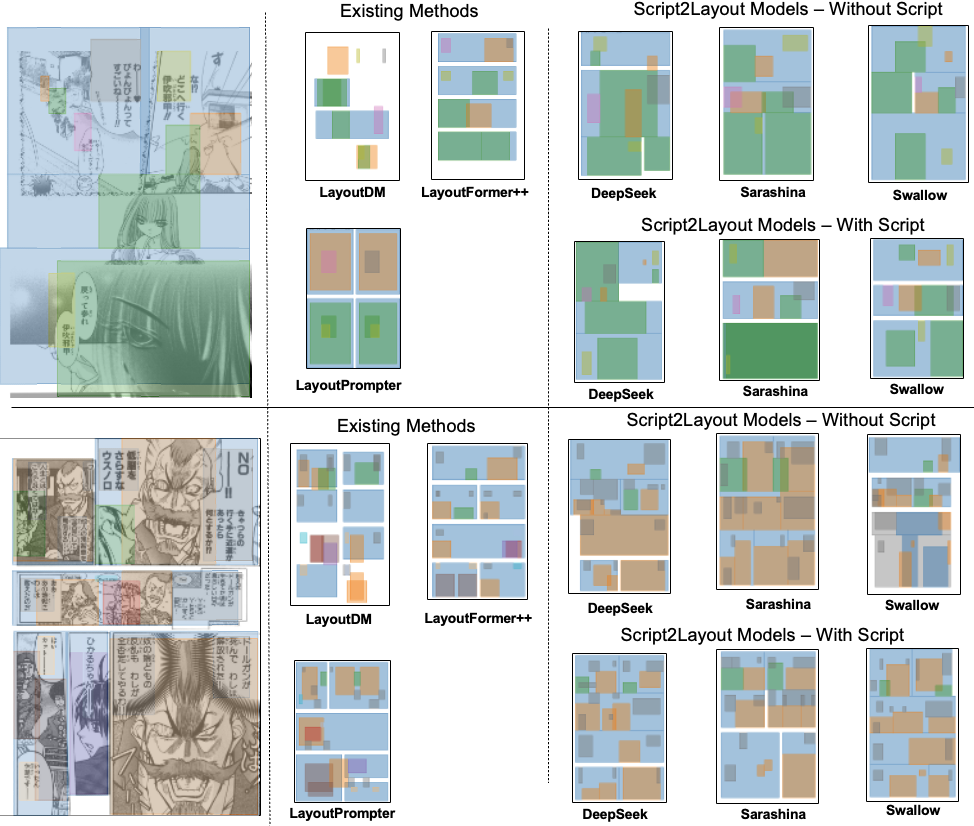
\includegraphics[width=\textwidth]{pict/04/evaluation_quality.png}

  \caption{
    Gen-T 条件下におけるレイアウト生成の可視化結果．
    各行に対して，左から順に
    正解レイアウト，
    既存手法の生成例，
    Script2Layoutの生成例，
    が並び，Script2Layoutでは上段にScript条件なし，下段にScript条件ありの結果を示す．(漫画: 上段『ヒーリング・プラネット』©桜野 みねね/エニックス，下段『ドールガン』©出口 竜正/秋田書店)
  }
  \label{fig:gen_t_qualitative}
\end{figure}

まず，既存手法と Script2Layout の生成結果を比較すると，コマ(水色の領域)の配置が，Script2Layout の方がより正解に近ししい傾向が見てとれる．例えば，1 行目の例では，正解のレイアウトにおいてコマがページを上段中段下段に分割するよう配置されているが，既存手法ではこれが再現されていない．一方で，Script2Layout ではこの傾向がより正確に捉えられている．また，目立たせるべきキャラクターの大きさについても，Script2Layout の方が正解に近しい傾向がみられる．例えば 2 行目の例では，正解レイアウトにおいて右下のキャラクター(オレンジ色の領域)が大きく描かれているが，既存手法ではこれが反映されていない．一方で，Script2Layout では配置の点では違いがみられるものの、このキャラクターを画面に大きく目立たせようとする傾向は見て取れる．セリフやキャラクター名の情報がこのようなコマ割りやキャラクターの重要度に関する配置設計に有効に働いた可能性を示唆している．

次に，Script2Layout における Script 条件の有無による違いを比較すると，Script 条件ありの方がキャラクター配置の点で，わずかに正解に近しい傾向が見てとれる．例えば，2 行目の例では，正解レイアウトにおいてオレンジ色の領域をもつキャラクターが，ページの上から順に登場しているが，Script 条件ありの生成例ではこれが再現されているようにみてとれる．一方で，Script 条件なしの生成例では，このキャラクターが特にページ下部に集中して配置されている．これは脚本情報にある文脈からこのキャラクターの登場を把握し，ページ全体にわたって適切に分散配置することが可能になったためと考えられる．

\subsection{Gen-TS 条件下での結果と考察:}
以下では，Gen-TS 条件下における定量的結果について考察する．本条件では，各要素の大きさがあらかじめ与えられているため，
Gen-T 条件と比較して幾何的制約が強く，
主に要素配置の相対位置関係の予測精度が問われる設定となっている．
そのため，生成結果の視覚的差異が相対的に小さくなり，
定性的比較から得られる追加的な知見は限定的であると考えられる．
また，漫画の制作を考慮してもこのような条件化での生成は実応用性が限定的であると考えられる．
以上を踏まえ，Gen-TS 条件においては
定量評価結果を中心に考察を行い，
生成結果の可視化による定性的評価は行わない．

表~\ref{tab:results_gen_ts} に，
Gen-TS 条件（要素のカテゴリとサイズを既知とする条件）における
レイアウト生成の定量評価結果を示す．

\begin{table*}[h]
  \captionsetup{font=small}
  \caption{
    Gen-TS 条件下におけるレイアウト生成の定量評価結果．
  }
  \vspace{-0.6em}
  \centering
  \label{tab:results_gen_ts}
  \setlength{\tabcolsep}{6pt}
  \begin{adjustbox}{max width=\textwidth}
    \begin{tabular}{l c c c c}
      \toprule
                                                      &
      \multicolumn{2}{c}{\textbf{Page-level metrics}} &
      \multicolumn{2}{c}{\textbf{Distribution-level metrics}}                                                                                                             \\
      \cmidrule(lr){2-3} \cmidrule(lr){4-5}
      \textbf{Model}                                  &
      mIoU $\uparrow$                                 & LTSim $\uparrow$                                    &
      FID $\downarrow$                                & \makecell{LTSim-MMD ($\times 10^{-2}$)$\downarrow$}                                                               \\
      \midrule

      \multicolumn{5}{l}{\itshape Existing Methods}                                                                                                                       \\
      LayoutDM
                                                      & 0.1890                                              & 0.7432             & \textbf{17.554}    & 0.263             \\
      LayoutFormer++
                                                      & 0.2034                                              & 0.7525             & \underline{18.058} & 0.378             \\
      LayoutPrompter
                                                      & 0.1326                                              & 0.7046             & 80.477             & 1.053             \\
      \midrule

      \multicolumn{5}{l}{\itshape Script2Layout（Without Script）}                                                                                                          \\
      DeepSeek
                                                      & \underline{0.3435}                                  & \underline{0.8145} & 19.981             & \textbf{0.052}    \\
      Sarashina
                                                      & 0.3165                                              & 0.8049             & 22.422             & 0.112             \\
      Swallow
                                                      & 0.3139                                              & 0.8042             & 20.977             & 0.108             \\
      \midrule

      \multicolumn{5}{l}{\itshape Script2Layout（With Script）}                                                                                                             \\
      DeepSeek
                                                      & 0.3429                                              & 0.8143             & 19.497             & \underline{0.057} \\
      Sarashina
                                                      & \textbf{0.3461}                                     & \textbf{0.8154}    & 19.426             & 0.078             \\
      Swallow
                                                      & 0.3431                                              & 0.8143             & 21.028             & 0.068             \\
      \bottomrule
    \end{tabular}
  \end{adjustbox}
\end{table*}

まず，既存のレイアウト生成手法と Script2Layout の
mIoU および LTSim に着目すると，
Gen-TS 条件下においても Script2Layout がすべての既存手法を大きく上回っていることが分かる．
例えば，mIoU では既存手法の最高値が LayoutFormer++ の 0.2034 であるのに対し，
Script2Layout はいずれのモデルにおいても 0.3100 以上を達成している．
サイズ情報が与えられた状況下においても，
Script2Layout がより正確な要素配置を実現できていることが示されている．
また，LTSim においても同様に，
Script2Layout は 0.800 を超える高い値を示しており，
ページ全体としての幾何的一貫性が大きく改善されている．
一方，FID に関しては，
LayoutDM が最良値を示していることがわかる．しかし，LTSim-MMD に関しては
いずれのScript2Layout も既存手法よりも良好な結果を示しており，
生成分布全体のもっともらしさについても既存手法には劣らないことが示唆される．

次に，Script2Layout における Script 条件の有無の影響を比較する．
Gen-TS 条件下では，
Script の有無による差は Gen-T 条件ほど顕著ではないが，
多くの指標において Script あり条件が
Script なし条件と同等，あるいはわずかに良好な値を示している．
特に LTSim-MMD においては，
すべてのモデルで Script あり条件が
より良好な値を示しており，
生成分布全体の安定性が向上していることが分かる．
この結果は，
サイズ情報という強い幾何的制約が与えられた状況では，
Script が要素配置の直接的な精度向上に与える影響は限定的となる一方で，
生成結果全体のばらつきを抑え，
分布としての一貫性を高める効果を依然として持つことを示唆している．

\paragraph{Gen-T 条件との比較による考察}
Gen-T 条件と比較すると，Script2Layout， 既存手法によらず，多くのモデルが
Gen-TS 条件において
mIoU および LTSim が大きく向上している。
これは，要素サイズ情報がレイアウト生成において極めて重要な役割を果たしていることを示唆する。
一方で，Gen-TS 条件下では，
Script 条件の有無による性能差が相対的に縮小していることから，
強い幾何的制約が与えられることで，
言語情報が果たす役割が補助的なものへと移行することが分かる．

以上より，
Script2Layout は，
幾何的制約が弱い場合（Gen-T）には Script 情報を積極的に活用して配置精度を向上させ，
幾何的制約が強い場合（Gen-TS）においては，
生成分布の安定化という形で Script 情報の効果を発揮する柔軟な手法であることが示唆される．

\subsection{考察のまとめと手法の課題}
本節では，脚本に基づく漫画レイアウト生成手法 Script2Layout について，
Gen-T および Gen-TS 条件下での定量的・定性的評価を通じて，
その有効性を検証した．
実験の結果，
脚本情報を条件として与えることで，
要素配置の精度やページ全体の幾何的一貫性が向上すること，
またその効果がモデル構造に依存せず一貫して観測されることを確認した．

一方，本研究の結果から，
脚本情報の効果は与えられる制約条件によって
異なる形で現れることも明らかになった．
Gen-T 条件のように幾何的制約が弱い設定では，
脚本情報が要素の重要度や配置のバランスに強く寄与し，
配置精度および分布的一貫性の双方を改善する傾向が見られた．
これに対し，
Gen-TS 条件のように要素サイズが既知である場合には，
脚本情報による配置精度の向上は限定的となり，
主に生成分布の安定化という形で効果が現れることが確認された．
このことは，
強い幾何的制約が与えられた状況では，
言語情報が果たす役割が補助的なものへと移行する可能性を示唆している．

以上のように脚本情報の有効性は確認されたものの，
脚本中のどの要素（キャラクターの登場頻度，セリフ量，ト書きの内容など）が
レイアウト決定にどの程度寄与しているかについては，
本研究では十分に分析できていない．
脚本内の情報と生成結果との対応関係を
より詳細に可視化・解析することは，
Script2Layout の挙動理解を深める上で
今後の重要な課題である．

% ▼▼▼ 仕掛け：main じゃないとき（単体のとき）だけ参考文献を表示 ▼▼▼
\ifdefined\ismain\else
  \printbibliography[title=参考文献]
\fi
% ▲▲▲▲▲▲▲▲▲▲▲▲▲▲▲▲▲▲▲▲▲▲▲▲▲▲▲▲▲▲▲▲▲▲▲▲

\end{document}